\section{Experimental Results}
\subsection{Datasets}

For the experiments we used the toy data and real world data, as shown in Table~\ref{table:dataset}.

\begin{table}[H]
\centering
\caption{Summary of Datasets}
\label{table:dataset}
\begingroup
\setlength{\tabcolsep}{4pt}
\renewcommand{\arraystretch}{1.35}
\begin{tabular}{|c|c|c|c|}
\hline
Graph          & n & $|E|$ & $\Delta(G)$\\ \hline
Small World Network (Newman\_watts\_strogatz\_graph) & 500 & 18025 &  1000\\ \hline
SNAP Facebook combined dataset~\cite{facebook_combine_data}  & 4039 & 88234 & 1612010\\ \hline
SNAP Twitter combined dataset~\cite{twitter_combined_data}  & 81306 & 1768149 & 13082506\\ \hline
\end{tabular}
\endgroup
\end{table}

\begin{figure}[H]
    \centering
    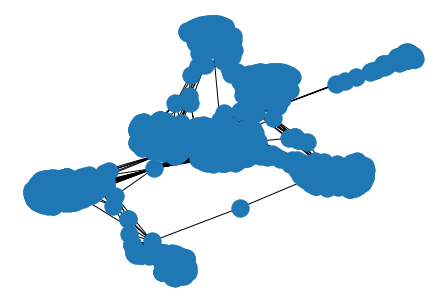
\includegraphics[width=10cm]{figs/facebook_data.png}
    \caption{SNAP (Stanford Large Network Datasets): Facebook Combined Dataset}
    \label{fig:facebook_dataset}
\end{figure}

\subsection{Hyper-parameters}
Probability of State 0 (Pro-vaccine) in initial Strategy Vector was kept at = 0.7.

\begin{table}[H]
\centering
\caption{Values of Hyper-parameters}
\label{table:hyper-params}
\begingroup
\setlength{\tabcolsep}{4pt}
\renewcommand{\arraystretch}{1.35}
\begin{tabular}{|c|l|}
\hline
Hyper-parameters          & Values\\ \hline
$\gamma$ & 0.7, 0.8, 0.9\\ \hline
$\delta$         & 0, 1, 2, 4\\ \hline
$\alpha$         & 1\\ \hline
$\beta$   & 1\\ \hline
$C$      & 1, 2, 4, 8~\cite{cvalue}\\ \hline
\end{tabular}
\endgroup
\end{table}

\subsection{Experimental Setup}
% In dataset 1, number of anti-vaccine nodes quickly diminishes to zero within <= 10 epochs.
% In dataset 2, both pro and anti vaccine sentiments co-exist in NE, within <= 20 epochs
% NE anti-vaccine fraction depends on initial x
% Usually < 0.01

% Changing $\alpha$, $\beta$ has no effect (which is evident from Lemma~\ref{lemma:alpha_beta_independence}).





\noindent
\textbf{Experiment 1:} We started with 100 different random configurations of the inital strategy vector, keeping the probability of initially being pro-vaccine fixed to 0.7. Fig.~\ref{fig:convergence_hist} shows the histogram of the time to reach the Nash Equilibrium using the SNAP dataset. As we can see from the figure, usually it takes around 3 or 4 epochs to reach the equilibrium. 

\begin{figure}[H]
    \centering
    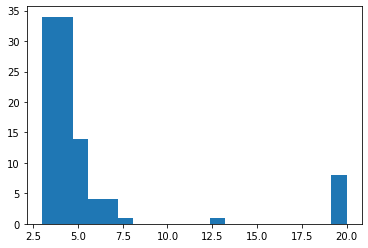
\includegraphics[width=12cm]{figs/convergence_hist.png}
    \caption{Histogram of number of epochs to reach NE}
    \label{fig:convergence_hist}
\end{figure}


Fig.~\ref{fig:exp1-diff-params} shows how the barplot changes as the hyper-parameters varry. As we can see from the figure, in this case also, in most cases, the number of epochs for convergence is less than 15.

\begin{figure}[H]
    \centering
    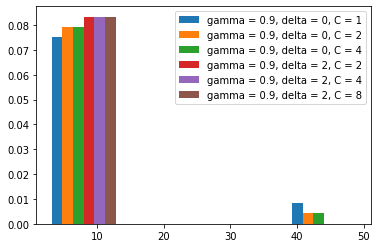
\includegraphics[width=12cm]{figs/exp1-diff-params.png}
    \caption{Histogram of number of epochs to reach NE starting with random initial strategy vector}
    \label{fig:exp1-diff-params}
\end{figure}




\begin{figure}[H]
    \centering
    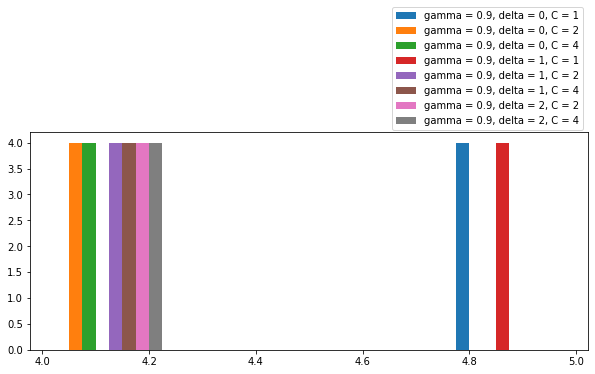
\includegraphics[width=14cm]{figs/exp1-diff-params-degree.png}
    \caption{Histogram of number of epochs to reach NE starting with highest degree nodes being anti-vaccine}
    \label{fig:exp1-diff-params-degree}
\end{figure}

\begin{figure}[H]
    \centering
    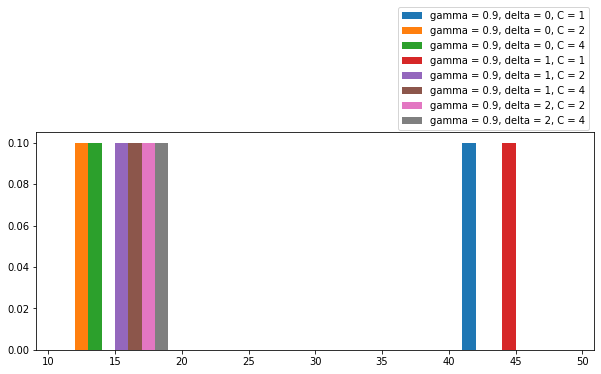
\includegraphics[width=14cm]{figs/exp1-diff-params-clusters.png}
    \caption{Histogram of number of epochs to reach NE starting nodes with highest clustering coefficients being anti-vaccine}
    \label{fig:exp1-diff-params-cluster}
\end{figure}



\noindent
\textbf{Experiment 2:} We start with the same initial strategy vector. We plot the number of unvaccinated nodes per epoch, until the network reaches an equillibrium. Fig.~\ref{fig:antivax_epoch} shows how the number of unvaccinated nodes varies with different parameters in the Facebook Combined dataset.

\begin{figure}[H]
    \centering
    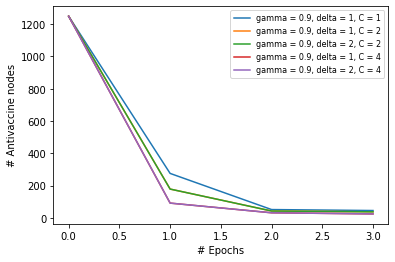
\includegraphics[width=12cm]{figs/exp1-random.png}
    \caption{Number of Antivaccine Nodes per epoch, varying the hyper-parameters}
    \label{fig:antivax_epoch}
\end{figure}


\begin{figure}[H]
    \centering
    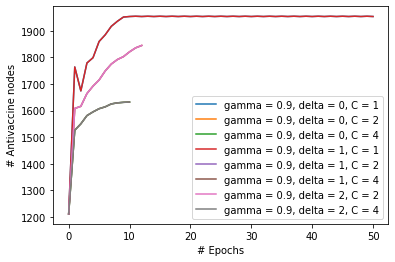
\includegraphics[width=12cm]{figs/exp2-diff-params-degree.png}
    \caption{Number of Antivaccine Nodes per epoch starting with highest degree nodes being anti-vaccine}
    \label{fig:exp2-diff-params-degree}
\end{figure}


\begin{figure}[H]
    \centering
    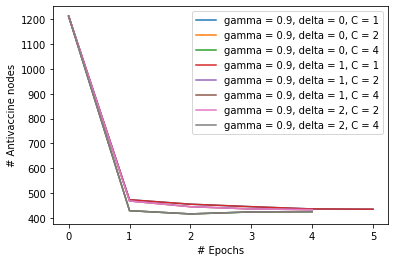
\includegraphics[width=12cm]{figs/exp2-diff-params-cluster.png}
    \caption{Number of Antivaccine Nodes per epoch, starting with nodes with highest clustering coefficient being anti-vaccine}
    \label{fig:exp2-diff-params-cluster}
\end{figure}



\noindent
\textbf{Experiment 3:} characteristics of nodes in NE: We look at the properties of nodes (e.g., degree, clustering coefficient) which end up in state 1 in experiment 2. Fig.~\ref{fig:antivax_degree} shows the histogram of the degrees of these nodes in the Facebook Combined dataset after starting with a random initial strategy vector with probability of being pro-vaccine being 0.7.

\begin{figure}[H]
    \centering
    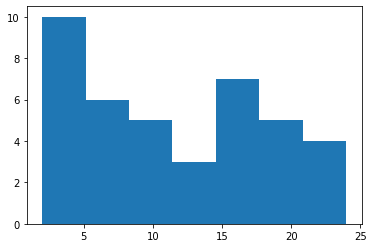
\includegraphics[width=12cm]{figs/antivax_degree.png}
    \caption{Histogram of degree of Anti-vaccine nodes in NE}
    \label{fig:antivax_degree}
\end{figure}


Fig.~\ref{fig:hist_boxplot_random}
% and~\ref{fig:boxplot_degree_cropped_1} through~\ref{fig:boxplot_degree_cropped_6} 
shows the average number of nodes having a particular degree, as well as the variance as a boxplot-- after the experiment is simulated 100 times with \textbf{random} initial strategy vectors with probability of being pro-vaccine being 0.6, $\alpha = \beta = \gamma = 1, C = 2 $ and $\delta = 0.9 $. 

\begin{figure}[H]
    \centering
    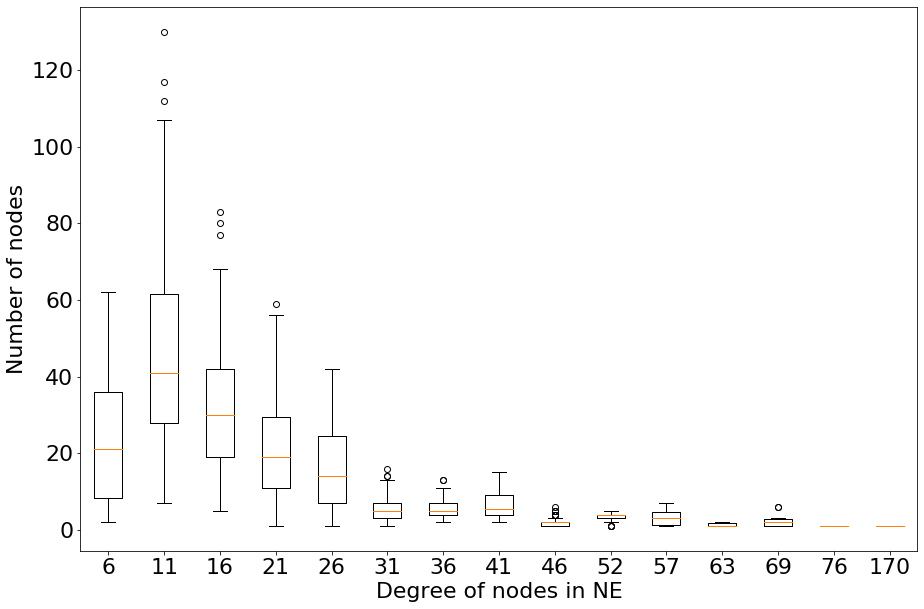
\includegraphics[width=14cm]{figs/exp3-random.png}
    \caption{Boxplot of degree of Anti-vaccine nodes in NE}
    \label{fig:hist_boxplot_random}
\end{figure}

\begin{figure}[H]
    \centering
    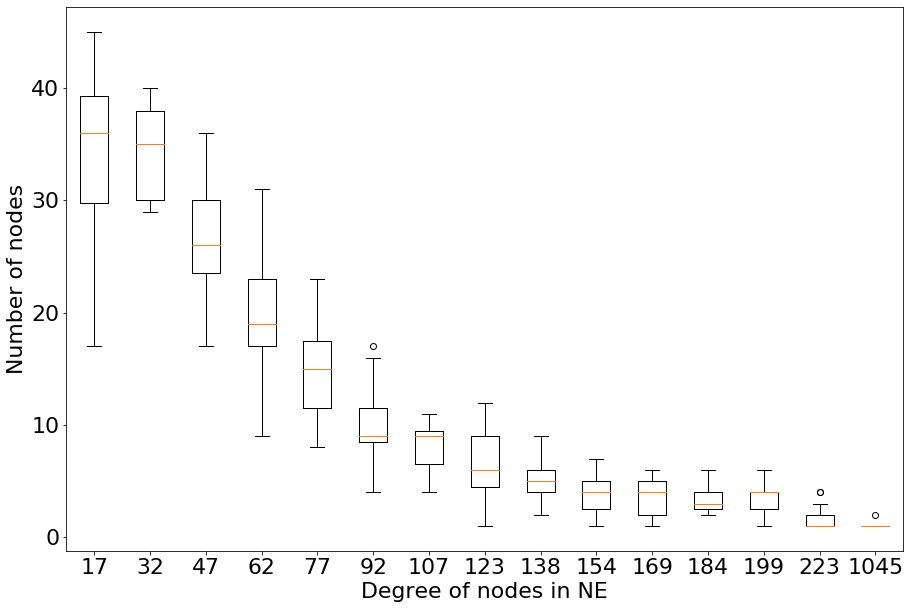
\includegraphics[width=12cm]{figs/exp3-degree.png}
    \caption{Boxplot of degree of Anti-vaccine nodes in NE, starting with highest degree nodes being anti-vaccine}
    \label{fig:exp3-degree}
\end{figure}

\begin{figure}[H]
    \centering
    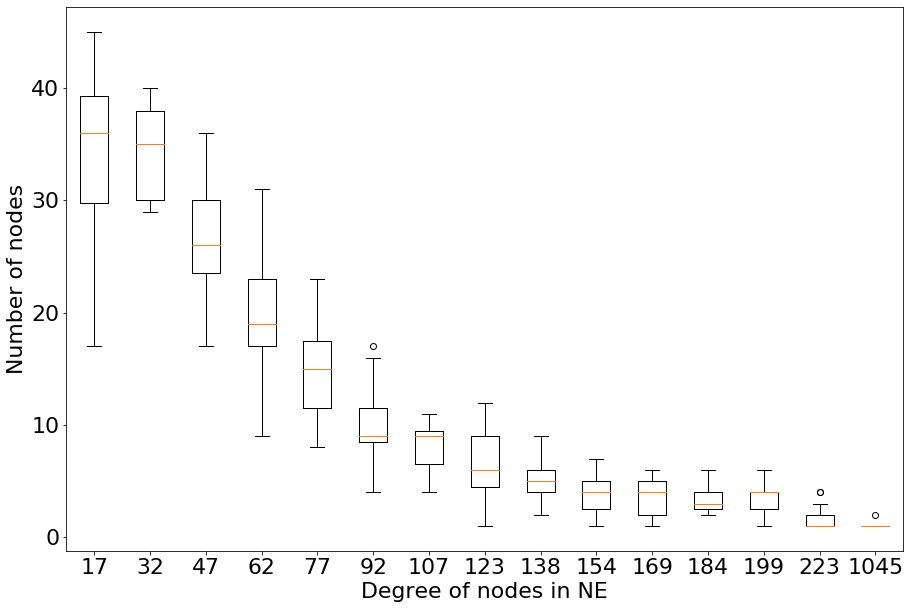
\includegraphics[width=12cm]{figs/exp3-degree.png}
    \caption{Boxplot of degree of Anti-vaccine nodes in NE, starting with nodes with highest clustering coefficient being anti-vaccine}
    \label{fig:exp3-cluster}
\end{figure}


% \begin{figure}[H]
%     \centering
%     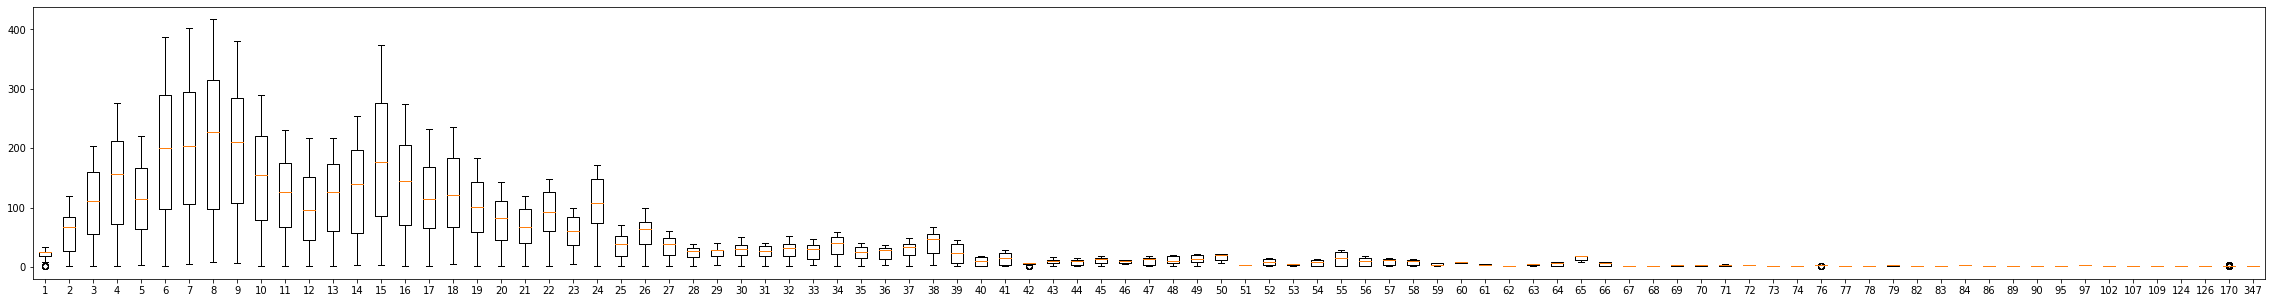
\includegraphics[width=15cm]{figs/boxplot.png}
%     \caption{Boxplot of degree of Anti-vaccine nodes in NE}
%     \label{fig:boxplot_degree}
% \end{figure}


% \begin{figure}[H]
%     \centering
%     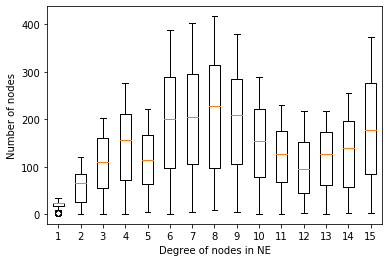
\includegraphics[width=10cm]{figs/box/1.png}
%     \caption{Boxplot of degree of Anti-vaccine nodes in NE}
%     \label{fig:boxplot_degree_cropped_1}
% \end{figure}

% \begin{figure}[H]
%     \centering
%     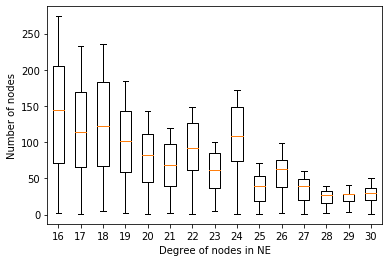
\includegraphics[width=10cm]{figs/box/2.png}
%     \caption{Boxplot of degree of Anti-vaccine nodes in NE}
%     \label{fig:boxplot_degree_cropped_2}
% \end{figure}

% \begin{figure}[H]
%     \centering
%     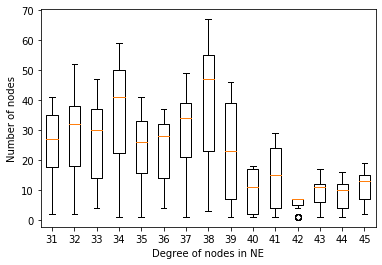
\includegraphics[width=10cm]{figs/box/3.png}
%     \caption{Boxplot of degree of Anti-vaccine nodes in NE}
%     \label{fig:boxplot_degree_cropped_3}
% \end{figure}

% \begin{figure}[H]
%     \centering
%     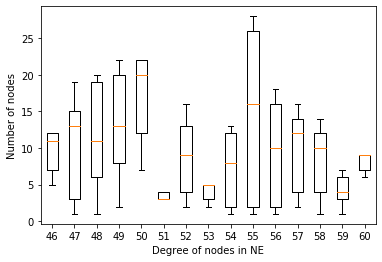
\includegraphics[width=10cm]{figs/box/4.png}
%     \caption{Boxplot of degree of Anti-vaccine nodes in NE}
%     \label{fig:boxplot_degree_cropped_4}
% \end{figure}

% \begin{figure}[H]
%     \centering
%     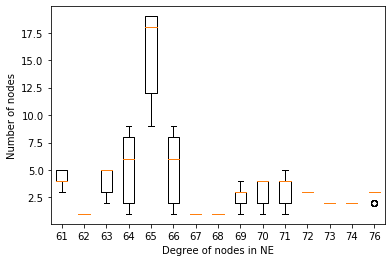
\includegraphics[width=10cm]{figs/box/5.png}
%     \caption{Boxplot of degree of Anti-vaccine nodes in NE}
%     \label{fig:boxplot_degree_cropped_5}
% \end{figure}

% \begin{figure}[H]
%     \centering
%     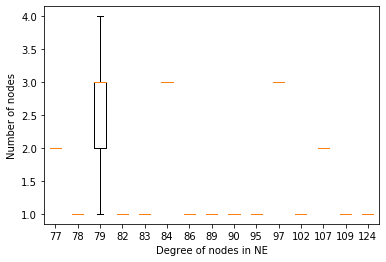
\includegraphics[width=10cm]{figs/box/6.png}
%     \caption{Boxplot of degree of Anti-vaccine nodes in NE}
%     \label{fig:boxplot_degree_cropped_6}
% \end{figure}



Fig.~\ref{fig:antivax_cluster_coeff} shows the histogram of the clustering coefficient of these nodes in the Facebook Combined dataset. As we can see, these nodes have relatively high clustering coefficients.


\begin{figure}[H]
    \centering
    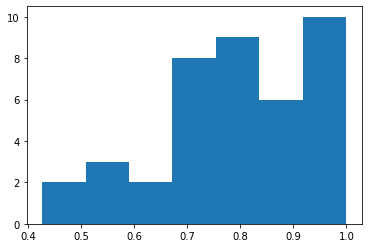
\includegraphics[width=12cm]{figs/antivax_cluster_coeff.png}
    \caption{Histogram of clustering coefficient of Anti-vaccine nodes in NE}
    \label{fig:antivax_cluster_coeff}
\end{figure}



% Experiment 4: Suppose we have some stubborn nodes S. These nodes are fixed in state 1, and their utility is not  improved by switching (this is a model). We can now see how the results in experiments 2 and 3 are affected by some stubborn nodes. There can be different strategies for picking stubborn nodes, e.g., by degree, or randomly within a community
\endinput